\documentclass[
  10pt
%, handout
]{beamer}

\usepackage{pgfpages}

\usepackage[T1]{fontenc}

%\setbeameroption{show notes on second screen}

\setbeamertemplate{section in toc}[sections numbered]

\usetheme[
  numbering=fraction
]{metropolis}
\usepackage{appendixnumberbeamer}

\usepackage{booktabs}
\usepackage[scale=2]{ccicons}

\usepackage{pgfplots}
\usepgfplotslibrary{dateplot}

\usepackage{xspace}
\newcommand{\themename}{\textbf{\textsc{metropolis}}\xspace}

\usepackage{graphicx}
\usepackage{listings}

\usepackage{lmodern}

\usepackage{eurosym}
\usepackage{amsmath, amssymb}
\usepackage[binary-units=true]{siunitx}
\DeclareSIUnit{\EUR}{\text{\euro}}

\usepackage{xcolor}
\newcommand\crule[3][black]{\textcolor{#1}{\rule{#2}{#3}}}
\definecolor{aswe-reactive}{cmyk}{1,0.9,0,0}
\definecolor{aswe-proactive}{cmyk}{0.6,0.9,0,0}
\definecolor{aswe-preferences}{cmyk}{0,0.75,1,0}
\definecolor{aswe-data}{cmyk}{0.85,0.1,1,0}

\setcounter{tocdepth}{1}  % Hide subsections in table of contents

% Content

\title{Introduction to Apache Cassandra}
\subtitle{}
\date{April 10, 2019}
\author{David Marchi, Daniel Schäfer, Erik Zeiske}
% \titlegraphic{\hfill\includegraphics[height=1.5cm]{logo.pdf}}

\begin{document}

\maketitle

\begin{frame}{Agenda}
  \tableofcontents[pausesections]
\end{frame}

\section{Overview}  % David

\begin{frame}{History}
  \begin{itemize}
    \item 2008, Developed by Facebook for inbox searching
    \item 2010, Proper Apache project
    \item Mainly developed and supported by Datastax
    \item 2019, 11th most popular database (db-engines.com)
  \end{itemize}
\end{frame}

\begin{frame}{Deployments}
  Widely used by large companies in big clusters:

  \begin{tabular}{@{}ll}
    \hline
    CERN    & Storage backend for ATLAS detector \\
    \hline
    Netflix & 2,500 nodes, 420 TB, over 1 trillion requests per day \\
            & Migrated from Oracle to Cassandra \\
    \hline
    eBay    & 6 billion writes and 5 billion reads daily \\
            & Single Cassandra table of 40TB \\
    \hline
    \onslide<2->
    Apple   & >75k Cassandra nodes with \textbf{10PB} in production \\
            & Several clusters with \textbf{1000+ nodes each!} \\
    \hline
  \end{tabular}

% https://cdsweb.cern.ch/record/1432912/files/ATL-DAQ-SLIDE-2012-067.pdf
% https://www.slideshare.net/adrianco/migrating-netflix-from-oracle-to-global-cassandra/28-Remote_Copies_Cassandra_duplicates_across
% https://www.slideshare.net/jaykumarpatel/cassandra-at-ebay-13920376
% https://www.datastax.com/resources/casestudies/ebay
\end{frame}

\begin{frame}{Properties}
  \begin{itemize}
    \item<1-> Wide Column Store
    \item<2-> Distributed and masterless Data Store
    \item<4-> Elastic scalability
    \item<5-> High Availability and Fault tolerance
    \item<6-> Tuneable Consistency
    \item<7-> Free software project of the Apache Foundation

  \end{itemize}
  \note<1>[item]{table-like but not relational; later more}
  \note<2>[item]{large data, distributed on commodity hardware}
  \note<3>[item]{masterless, no single point of failure}
  \note<4>[item]{add another machine, cassandra will adapt it}
  \note<5>[item]{Replace failed nodes with not downtime}
  \note<5>[item]{Replicate data to multiple data centers}
  \note<6>[item]{reffered to as "eventual conistent"}
  \note<7>[item]{Originally developed by Facebook in 2008, co-author Amazon DynamoDB}
\end{frame}

\section{Wide Column Store}  % David
\begin{frame}{Wide Column Store}
  \begin{itemize}
    \item<1-> Tabular but not relational
    \item<2-> \textbf{NOT} column oriented! Rows are stored together
    \item<3-> A row can have missing columns (Not stored on disk $\rightarrow$ sparse)
    \item<4-> Like key-value store where the value can have a subset of a predefined set of columns
  \end{itemize}

  \onslide<5->
  Interpretation of the name: \\
  Key value store with wide (complex) values that consist of columns

  \onslide<6->
  "Sparse, distributed multi-dimensional sorted map"
  % Chang, F., Dean, J., Ghemawat, S., Hsieh, et al. (2008). Bigtable: A distributed storage system for structured data. ACM Transactions on Computer Systems (TOCS), 26(2), 4

  \note<2>[item]{Unlike Vertica or SAP HANA}
  \note<6>[item]{Quote from original paper}
\end{frame}

\begin{frame}{Wide Column Store}
  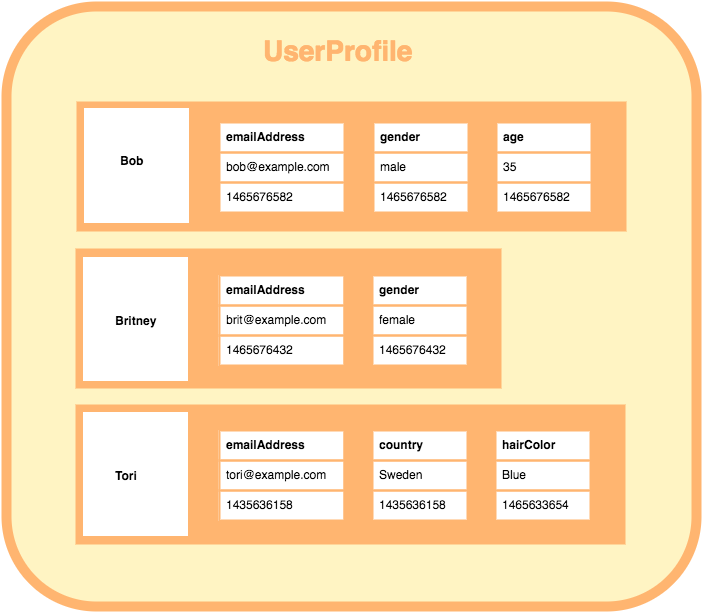
\includegraphics[width=0.75\columnwidth]{resources/wide_column_store.png}
\end{frame}

\section{Use-Cases Cassandra is (not) suited for}  % David
\begin{frame}{Pros and cons}
  \begin{columns}[T]
    \onslide<+->
    \begin{column}{0.55\textwidth}
      \underline{Use if you want/need}

      \begin{enumerate}[\textbf{\textcolor{aswe-data}{+}}]
        \item<+-> Fast writes \\ (high throughput, not latency)
        \item<+-> High availability
        \item<+-> Easy (linear) horizontal scalability
        \item<+-> No master $\rightarrow$ \\ Read from and write to any node
        \item<+-> Flexible schema \\ (rows can have missing columns)
        \item<+-> Globally distributed cluster
        \item<+-> Query language similar SQL (CQL)
      \end{enumerate}
      \note[item]{Writes include \lstinline{INSERT} \lstinline{UPDATE} \lstinline{DELETE}}
      \note[item]{Inter-node communication doesn't increase with more nodes}
      \note[item]{Missing columns aren't even saved to disk (sparse)}
    \end{column}

    \onslide<+->
    \begin{column}{0.45\textwidth}
      \underline{Don't use if you want/need}

      \begin{enumerate}[\textbf{\textcolor{aswe-preferences}{-}}]
        \item<+-> Single system instance
        \item<+-> Ever changing queries
        \item<+-> Lots of updates and deletes interspersed with reads
        \item<+-> Transactions (ACID)
        \item<+-> Relations (joins, ...)
        \item<+-> Column aggregation (\lstinline{GROUP BY})
        \item<+-> \lstinline{AUTO INCREMENT}
        \item<+-> Data validation / constraints (e.g. \lstinline{NULL} constraint, uniqueness)
      \end{enumerate}
      \note[item]{Cassandra is \textbf{NOT} column oriented}
    \end{column}
  \end{columns}
\end{frame}

\begin{frame}{General UseCase Conditions}
%Abstract UseCases
 \begin{itemize}
    \item<1-> Large Deployments
    \item<2-> Lots of writes, like a lot a lot
      \begin{itemize}
        \item<3-> "high performance at high write volumes with many concurrent client threads"
      \end{itemize}
    \item<4-> Geographical distribution
    % TODO: Think about this
    \item<5-> Evolving applications
 \end{itemize}

    % TODO fix numbering
    \note<1>[item]{Ingenuiety, architecture and featureset limited when used as single-node}
    \note<1>[item]{Several nodes? -> might be a fit}
    \note<1>[item]{Dozen of nodes? -> great fit}
    \note<2>[item]{Consider read / write ratio}
    \note<2>[item]{As mentioned, cassandra optimized for write throughput}
    \note<2>[item]{Not many updates / data changes, slows read down}
    \note<3>[item]{Configure to replicate across multiple data centers}
    \note<3>[item]{Globally deployed application}
    \note<3>[item]{Flexible schema, database evolves with application}

\end{frame}

\begin{frame}{Suitable usecases}
  Concrete use-cases
  \begin{itemize}
    \item Recording of transactions
      \begin{itemize}
        \item Shopping cart
        \item User transactions
      \end{itemize}
    \item Time series data
      \begin{itemize}
        \item Logs of any kind, e.g. sensors with huge outputs
        \item IoT
        \item User / Behavioural analytics
      \end{itemize}
    \item \textbf{Social media input and analysis}
  \end{itemize}

  \note[item]{Since it was developed to solve Facebook Inbox problem}

\end{frame}

\section{How to use CQL}  % Erik

\subsection{API Definition}
\subsection{CQL v. SQL}
\subsubsection{Creating a database(keystore)}
\begin{frame}[fragile]{Creating a database (keystore)}
  \begin{semiverbatim}
/* Create a new keyspace in CQL */
CREATE KEYSPACE data WITH replication =
\{'class': 'SimpleStrategy', 'replication_factor': 1\};

/* Create a new database in SQL */
CREATE DATABASE data;
  \end{semiverbatim}
\end{frame}

\subsubsection{Create Table}

\begin{frame}[fragile]{Create Table}
  \begin{semiverbatim}
CREATE TABLE groups (
   group_location varchar,
   added_date date,
   username varchar,
   PRIMARY KEY (...)
);
  \end{semiverbatim}
\end{frame}

\begin{frame}[fragile]{Primary Key}
  \begin{semiverbatim}
      parition key       clustering key  clustering key
       |       |                |            |
((groupname, group_location), added_date, username)
                                |
                            ORDER BY
  \end{semiverbatim}
\end{frame}

\begin{frame}{Cassandra API}
  \begin{itemize}
    \item insert(table, key, rowMutation) \\
          \only<2->{\lstinline{UPDATE table SET rowmutation WHERE key}}
    \item get(table, key, columnName) \\
          \only<3->{\lstinline{SELECT columnName FROM table WHERE primaryKey = key}}
    \item delete(table, key, columnName) \\
          \only<4->{\lstinline{DELETE columnName FROM table WHERE key}}
  \end{itemize}
\end{frame}

\subsubsection{Insert/Update Data}
\begin{frame}[fragile]{Insert/Update Data}
  What is the difference of the statements?
  \begin{semiverbatim}
/* Inserting Data */
INSERT INTO Person (lastname, name, email)
VALUES ('Musterfrau', 'Maxi', 'maxi@gmail.com');

/* Updating Data */
UPDATE Person SET email = 'maxi@gmail.com'
WHERE lastname='Musterfrau' AND name = 'MAXI';
  \end{semiverbatim}
  \only<2->{There is no difference. \textbf{Insert = Update}}
\end{frame}

\subsubsection{Delete Data}
\begin{frame}[fragile]{Delete Data}
  \begin{semiverbatim}
/* Deleting Data */
DELETE FROM Person
  WHERE lastname='Musterfrau' AND name = 'Maxi';
  \end{semiverbatim}
\end{frame}

\section{How to model data (or rather tables)}  % David

\begin{frame}{How to model data - Assumptions}
  \begin{itemize}
    \item Writing is cheap
    \item You have a lot of disk space
    \item Inter-node communication is expensive
  \end{itemize}
\end{frame}

\begin{frame}{How to model data - Constraints}
  \begin{itemize}
    \item<+-> No joins
    \item<+-> No referential integrity
    \item<+-> Denormalization
    \item<+-> Query-first design
    \item<+-> Sorting, design decision
  \end{itemize}
  % TODO - extensive notes
\end{frame}

\begin{frame}{How to model data - Example}
  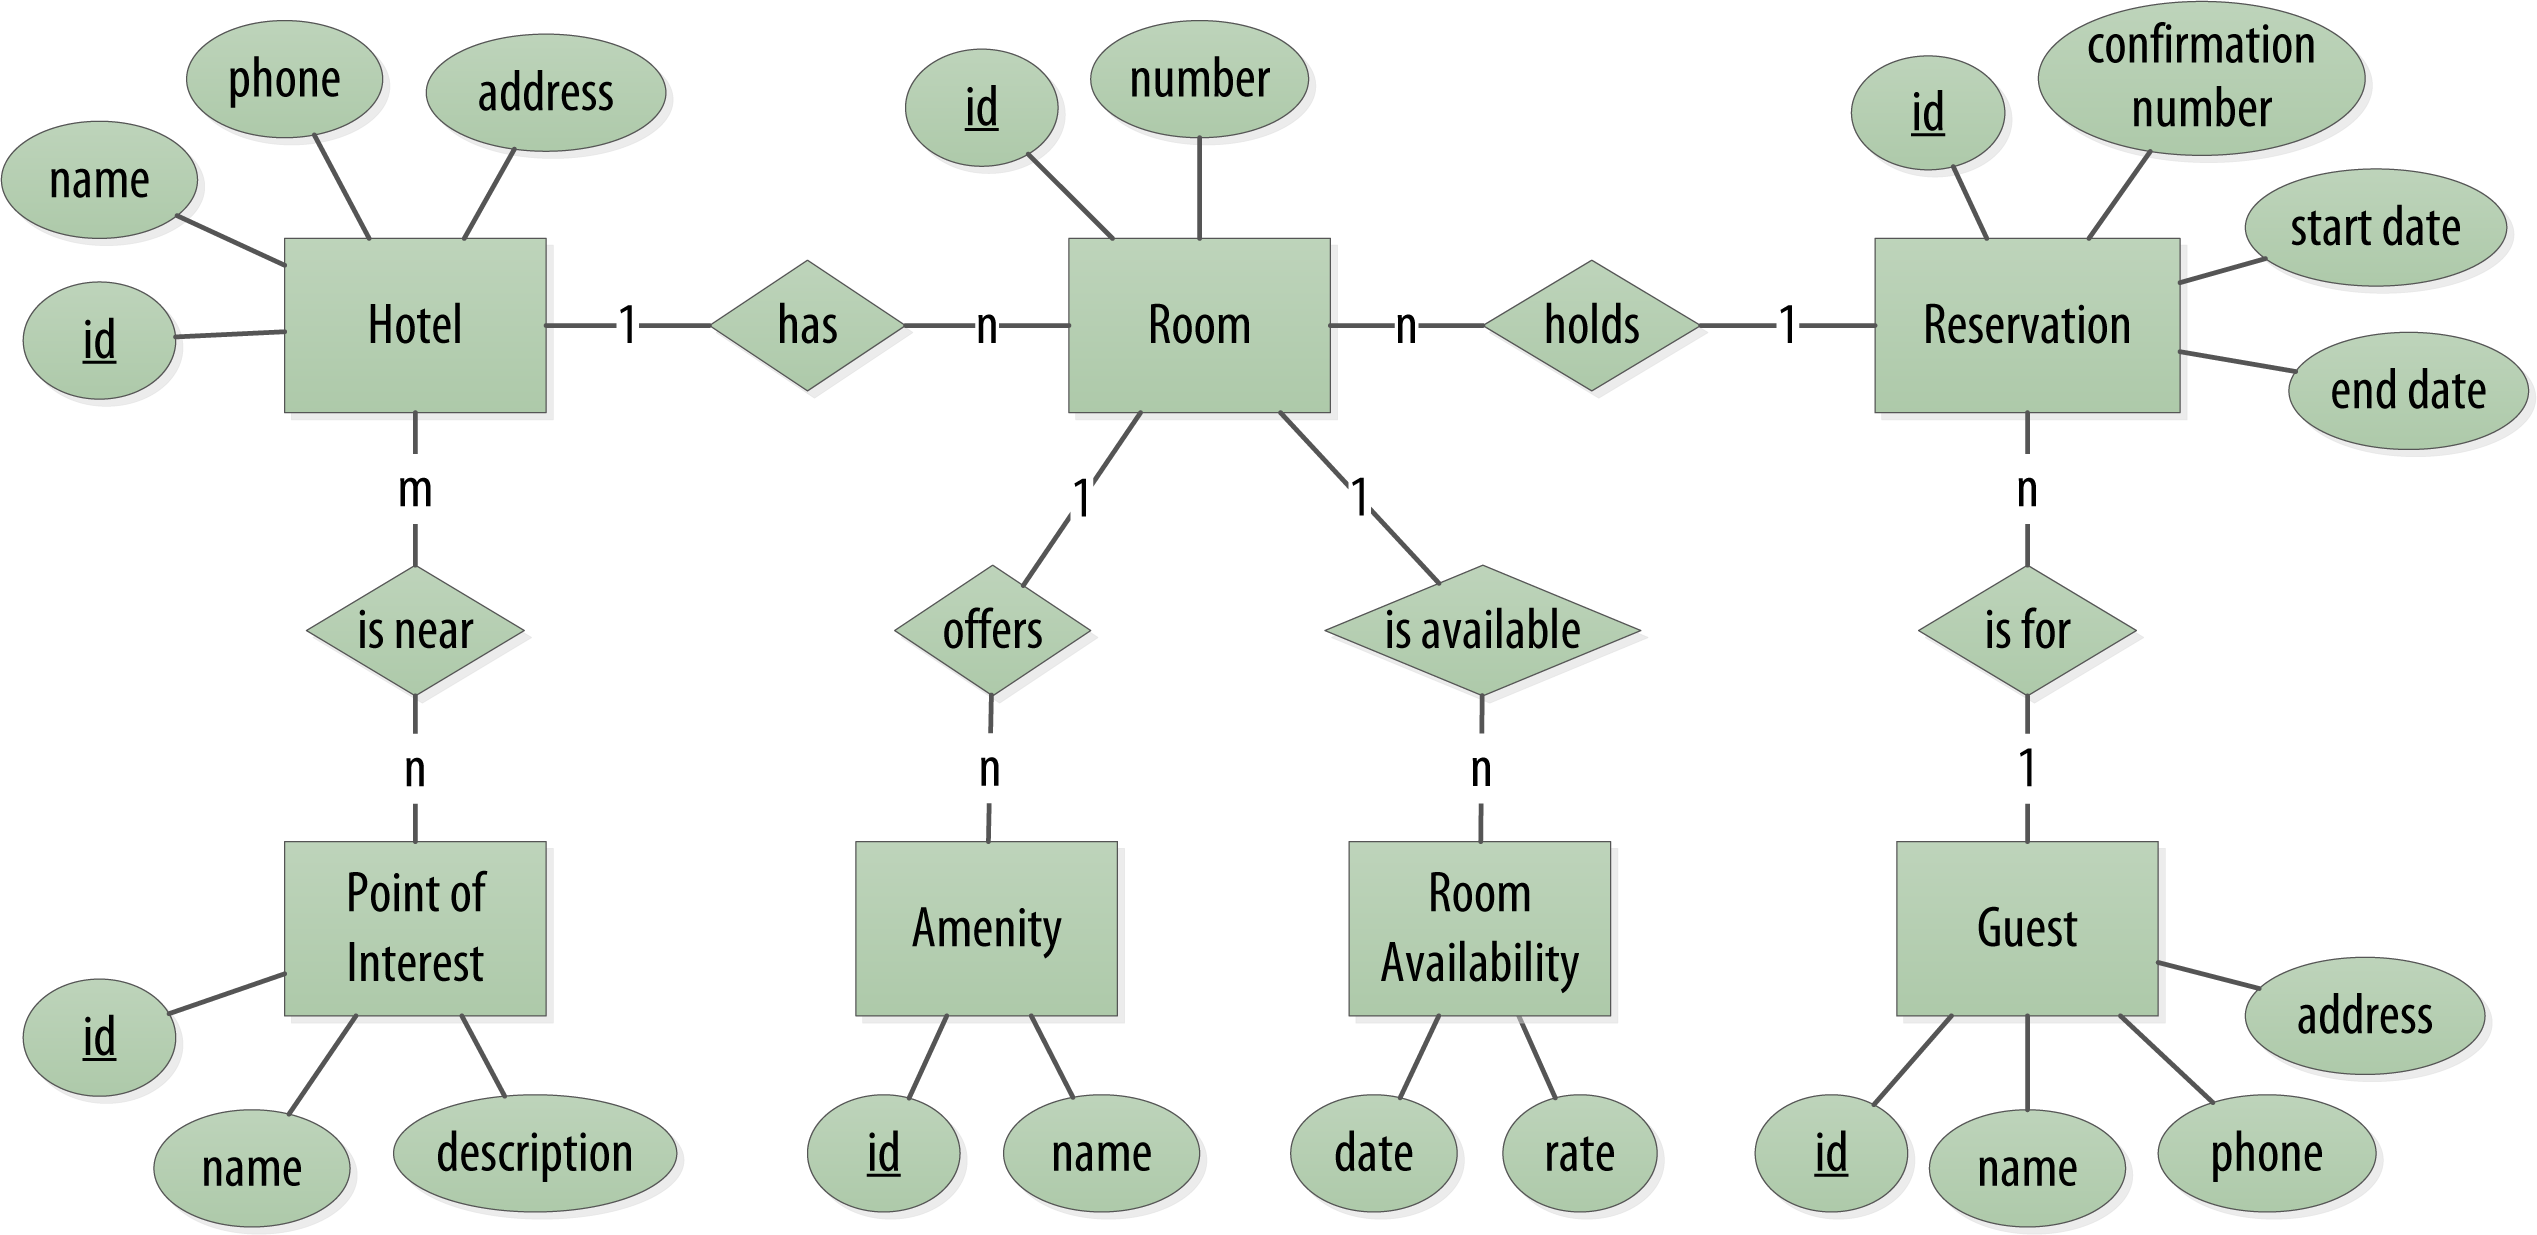
\includegraphics[width=0.75\columnwidth]{resources/model_example_entity_relation_step0.png}
\end{frame}

\begin{frame}{How to model data - Example}
  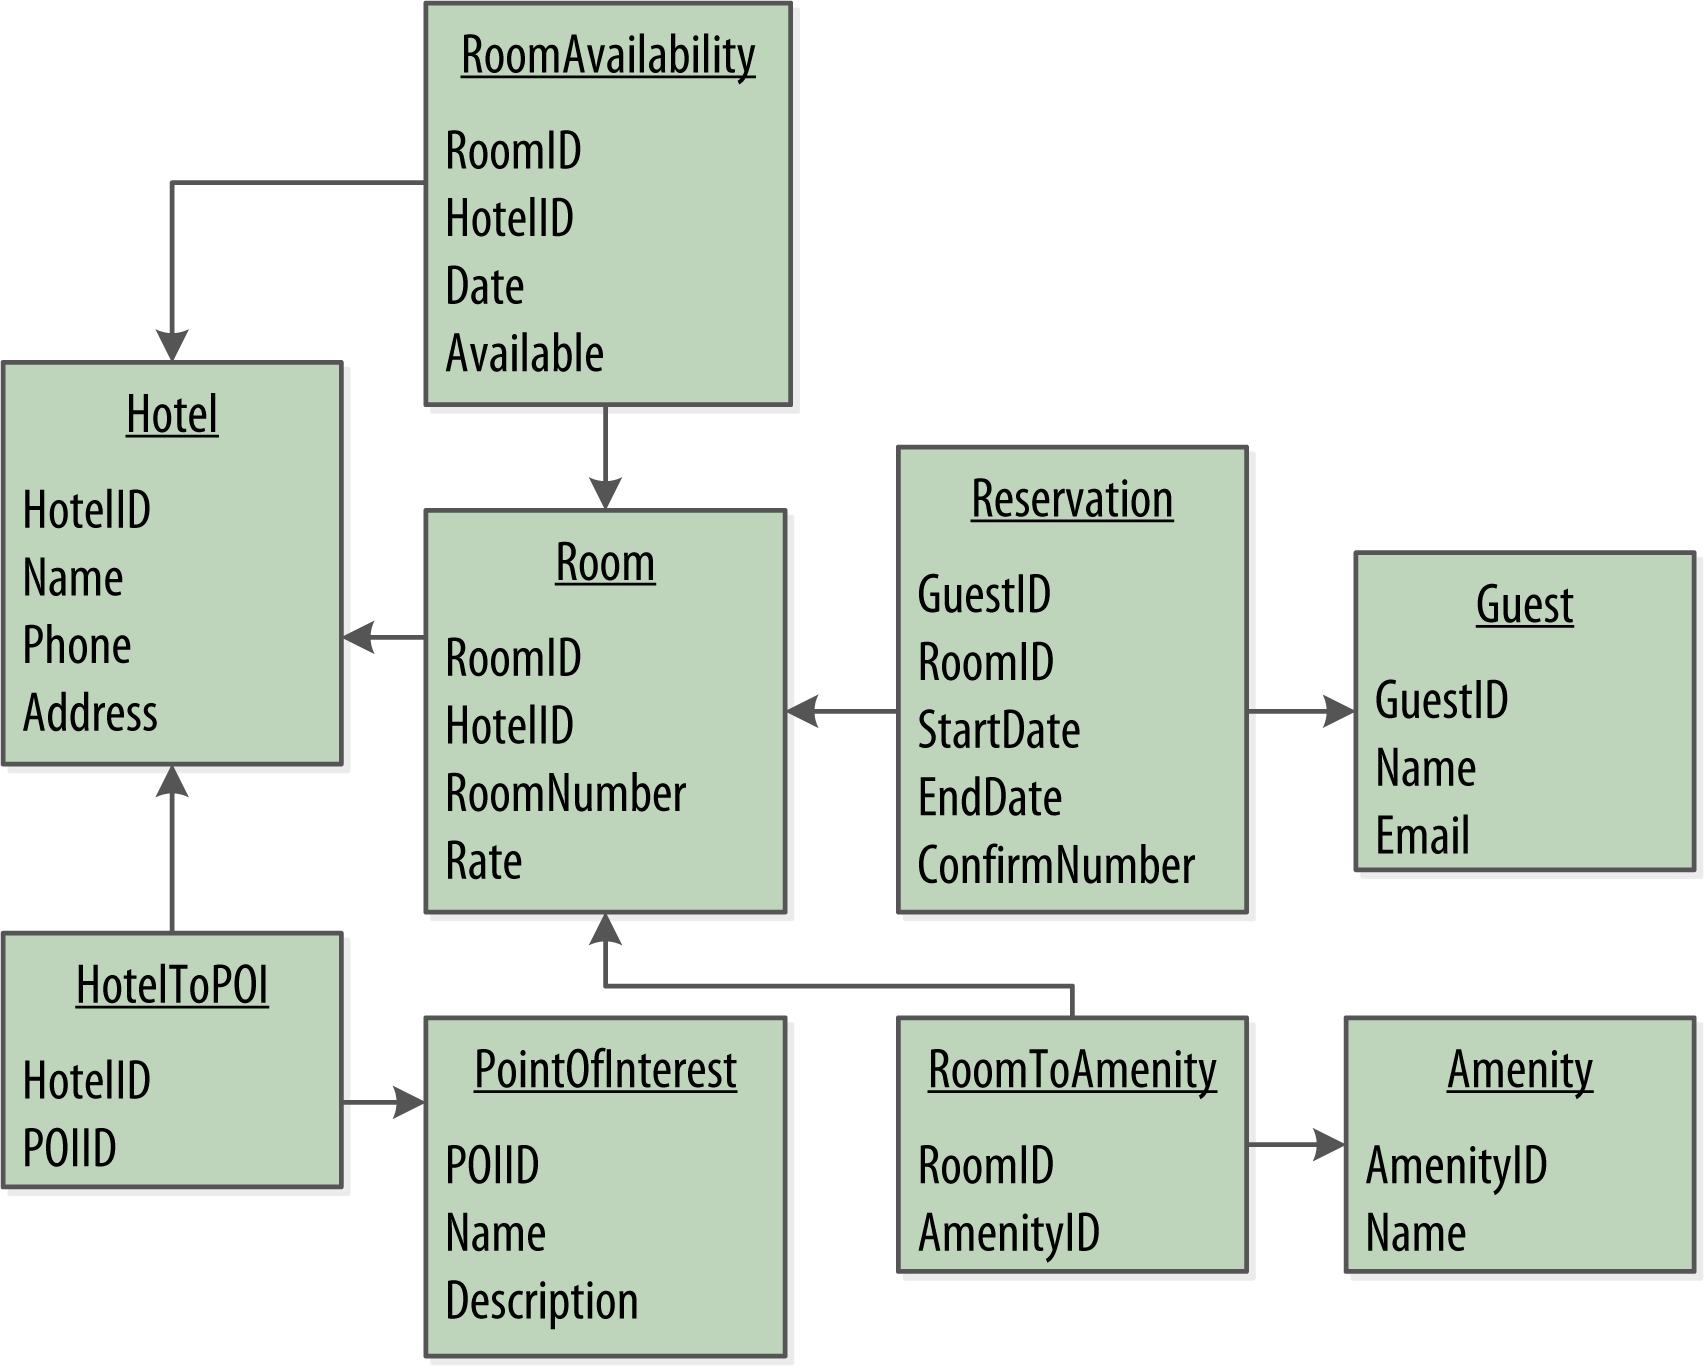
\includegraphics[width=0.75\columnwidth]{resources/model_example_rdbms_step1.png}
\end{frame}

\begin{frame}{How to model data - Example}
  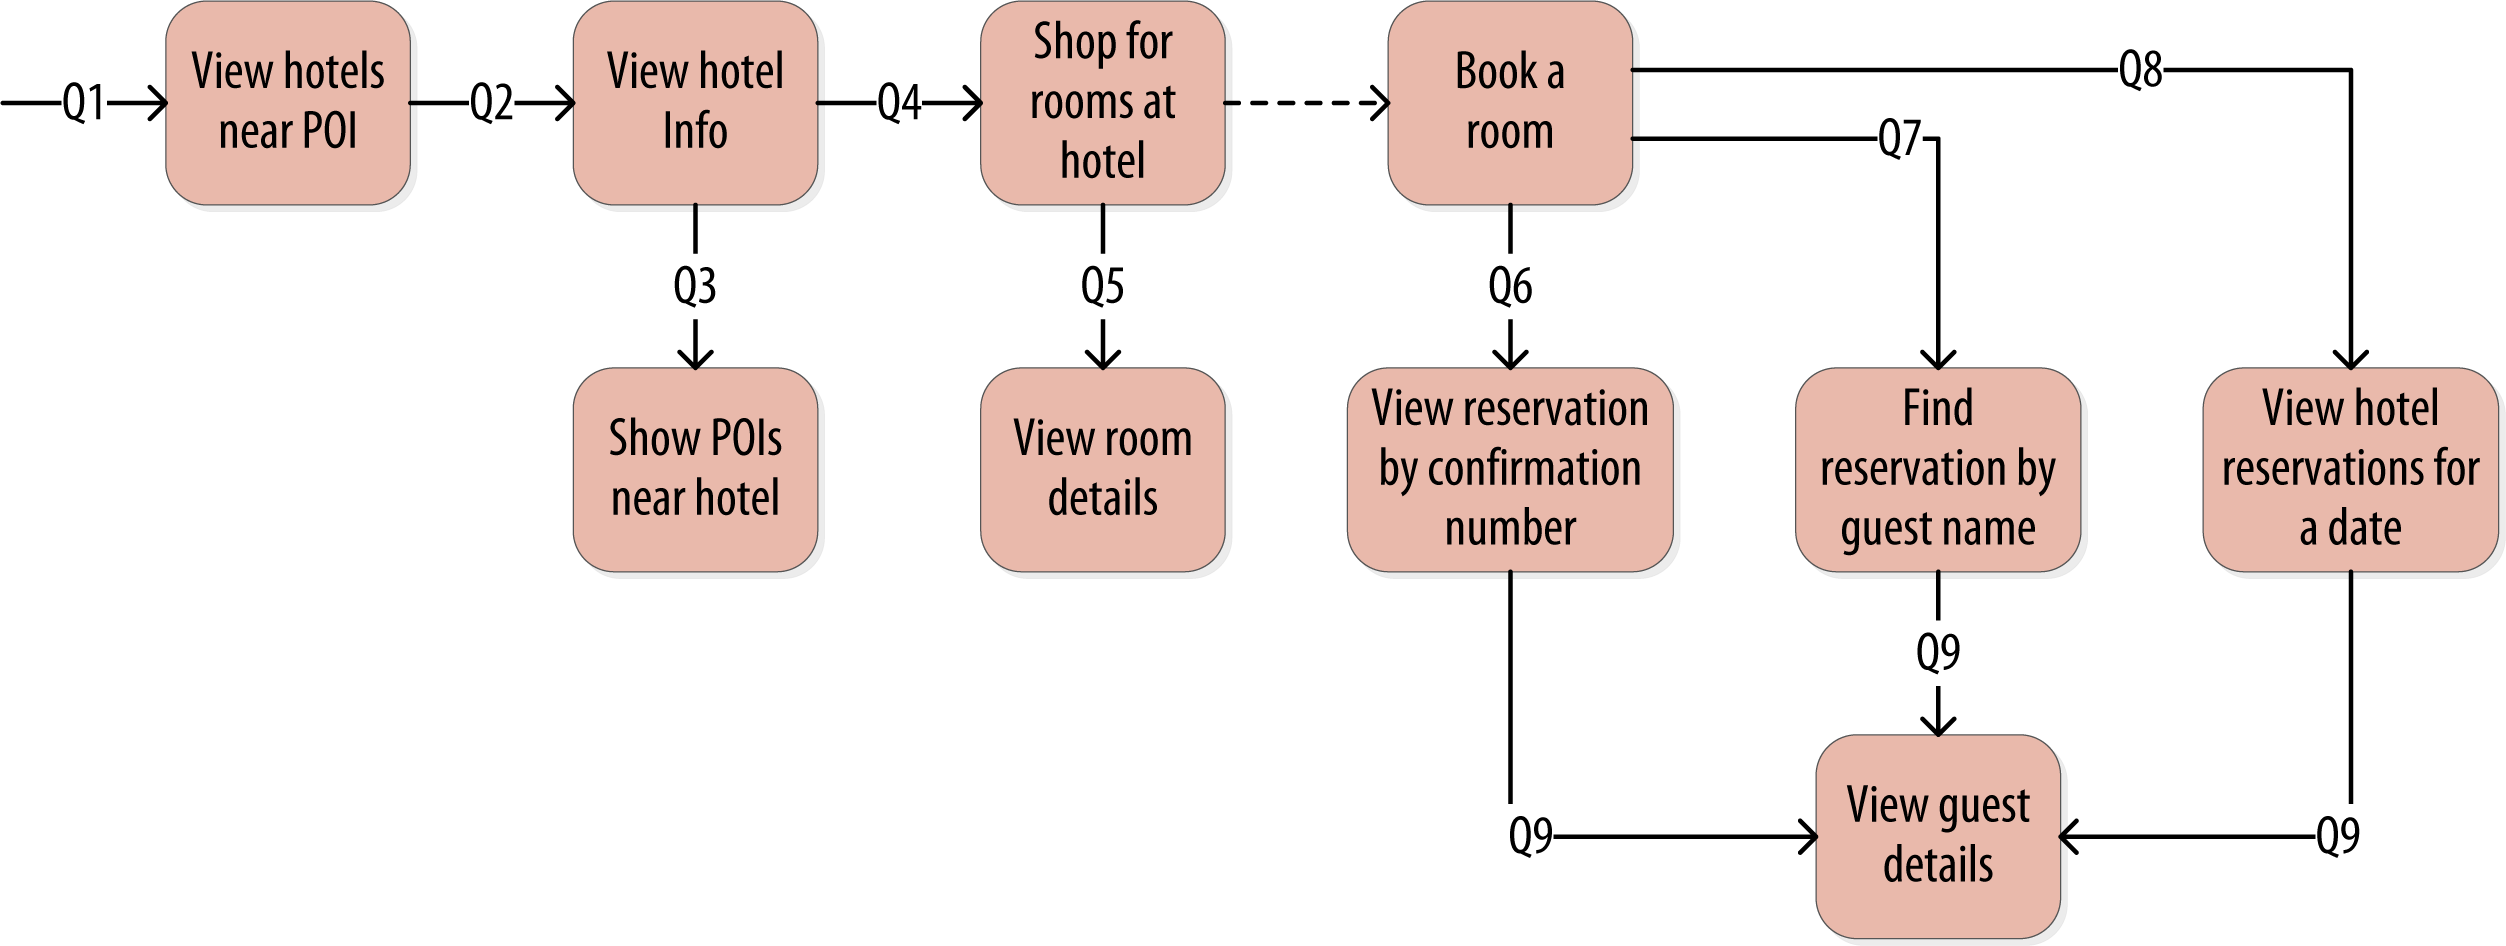
\includegraphics[width=0.75\columnwidth]{resources/model_example_queries_step2.png}
\end{frame}

\begin{frame}{How to model data - Chebotko Diagram}
  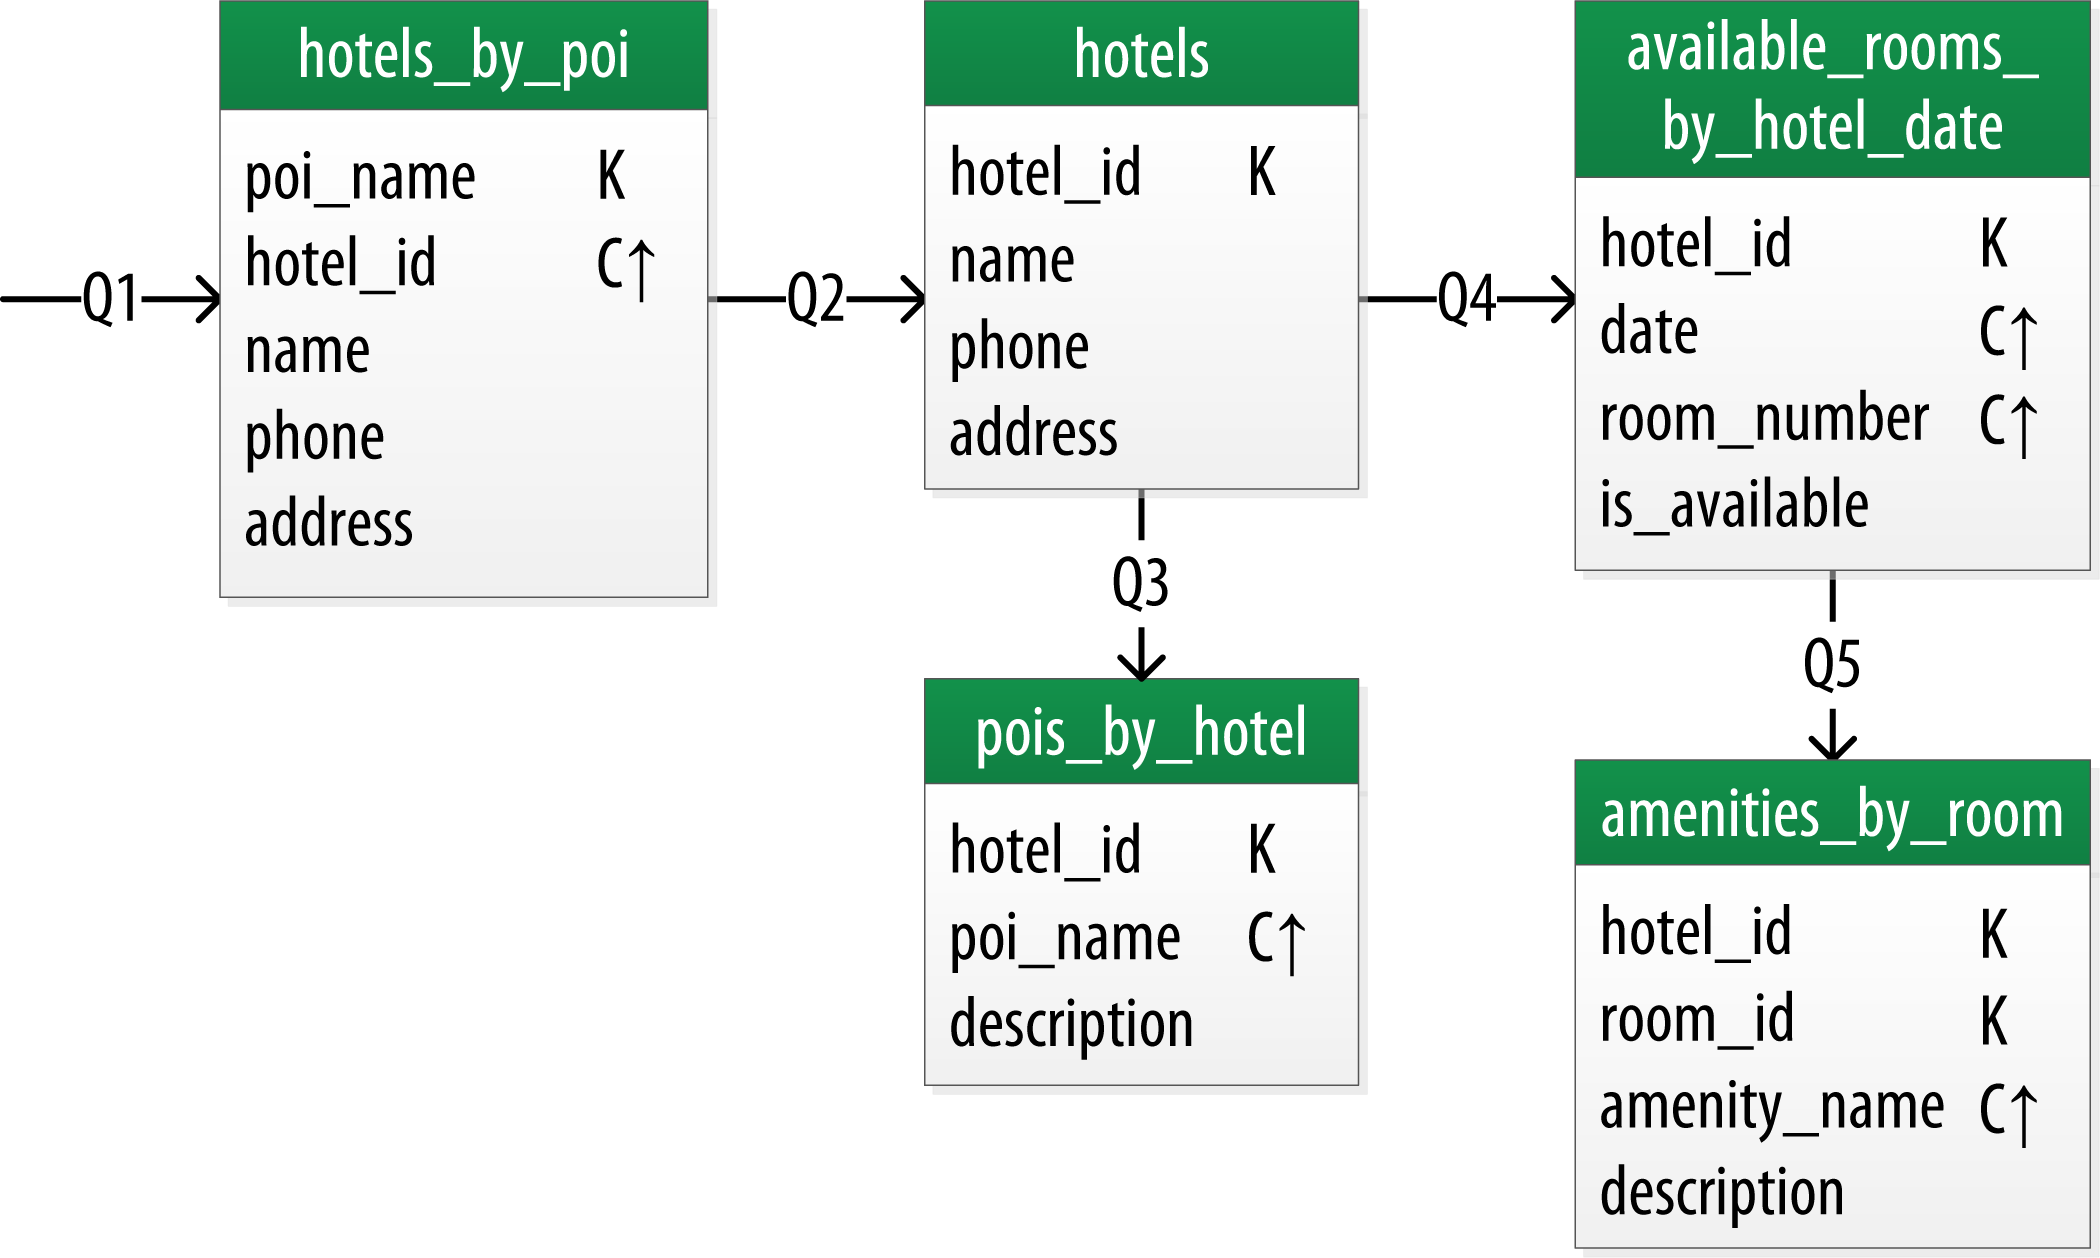
\includegraphics[width=0.75\columnwidth]{resources/model_example_chebotko_step3.png}
\end{frame}

% Rework slide / make a summary, point out differences
\begin{frame}{How to model data}
  \begin{itemize}
    \item Denormalize!
    % Writing and reading will be cheap - there are no joins
    \item Choose a good partition key
      \begin{itemize}
        \item Spread data evenly
        \item Optimize queries (tables) to read from few partitions
      \end{itemize}
    \item Model table to fit your queries
  \end{itemize}
\end{frame}

\subsection{Secondary index}  % Daniel

\begin{frame}[fragile]{Secondary index - Why}
  Make it possible to filter by a non primary-key column
  \onslide<1->
  \begin{semiverbatim}
  \onslide<2->
  cqlsh:db> CREATE TABLE users (
  cqlsh:db>  username varchar PRIMARY KEY,
  cqlsh:db>  age int
  cqlsh:db> );
  cqlsh:db> SELECT * FROM users WHERE age = 5;
  \onslide<4->
  cqlsh:db> \textcolor{red}{InvalidRequest: [might filter data]}
  \onslide<4->
  cqlsh:db> CREATE INDEX ON users (age);
  cqlsh:db> SELECT * FROM users WHERE age = 5;

   username | age
   \--\--\--\--\--\--\--\--\--+\--\--\--\--
      timmy |   5
  \end{semiverbatim}
  \note<2-3>[item]{Unpredicatable performance $\rightarrow$ ALLOW FILTERING}
  \note<2-3>[item]{Has to go through all nodes and all of their data}
\end{frame}

\begin{frame}{Secondary index - Implementation}
  % https://www.datastax.com/wp-content/uploads/2017/01/Native2i-Distributed-Index-3.png
  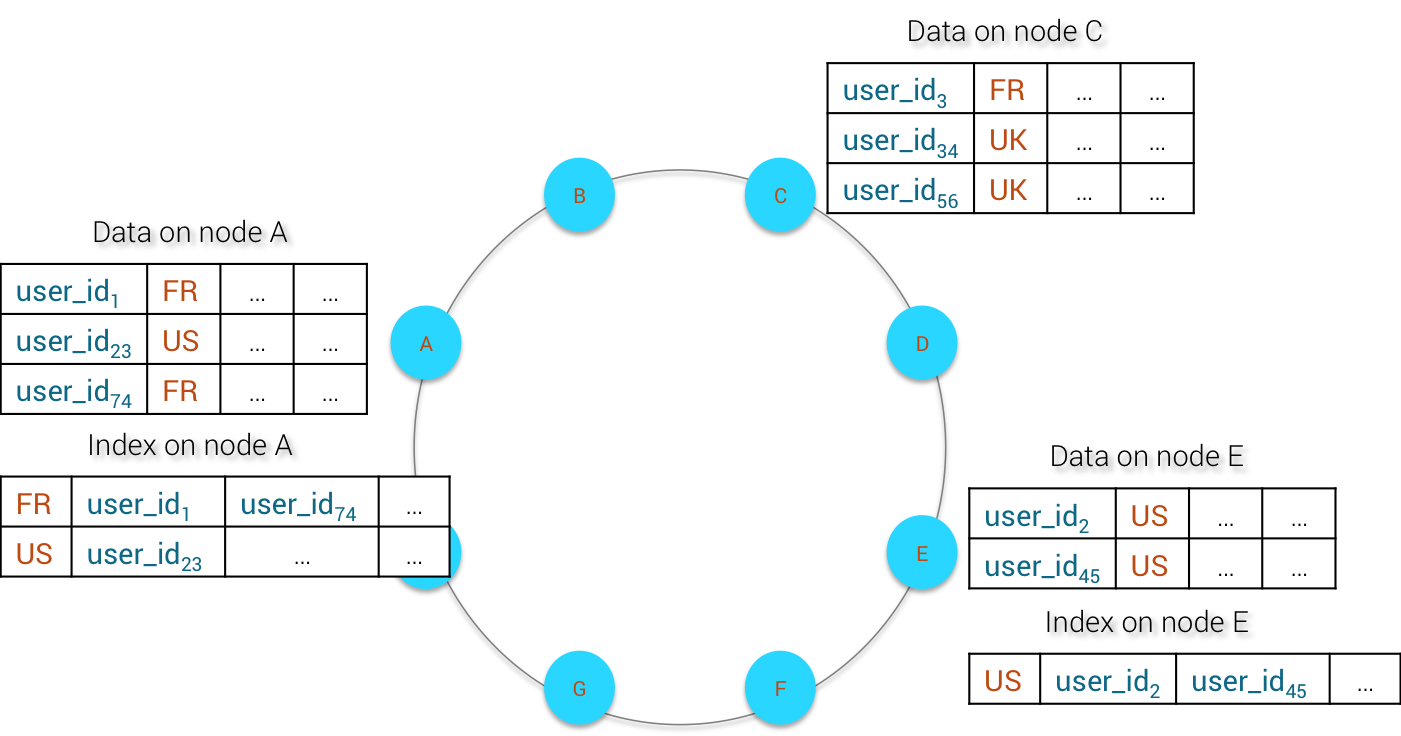
\includegraphics[width=1.0\textwidth]{resources/distributed_index.png}
  \note[item]{NOT tree, regular table}
  \note[item]{Distributed, same location as data}
  \note[item]{Restrict partition key $\rightarrow$ Find node}
  \note[item]{Heuristic to fetch data from likely nodes in stages}
\end{frame}

\begin{frame}{Secondary index - Summary}
  \begin{itemize}
    \item<1-> Distributed table with different primary key
    \item<2-> Located on same node as indexed data
      \begin{itemize}
        \item Fast to update
        \item Partitions as balanced as data
      \end{itemize}
    \item<3-> Good practice to restrict partition key as well
    \item<4-> Uses heuristic to fetch data from likely nodes $\rightarrow$ \textbf{Use LIMIT}
  \end{itemize}
  \note<3>[item]{Partition key $\rightarrow$ only needs to search single node}
\end{frame}

\begin{frame}{Secondary index - When not to use}
  Avoid columns
  \begin{itemize}
    \item<1-> with very high cardinality (e.g. user id)
    \item<2-> with very low cardinality (e.g. country name)
    \item<3-> that are updated/deleted very frequently
  \end{itemize}
  \note<1>[item]{Low chance of finding - no partition key $\rightarrow$ queries all nodes}
  \note<2>[item]{Results in huge index rows}  % TODO: Think about a good explanation
  \note<3>[item]{Updates have to update two tables}
  \note<3>[item]{Tombstones are stored in index - hard limit of 100K $\rightarrow$ Query FAILS}
\end{frame}

\section{Local reads and writes}  % Erik
\begin{frame}{Write process}
  \begin{center}
    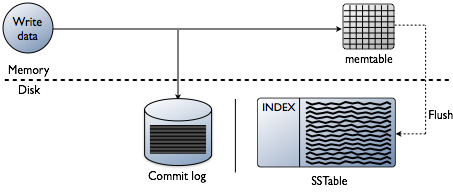
\includegraphics[width=0.75\textwidth]{resources/local_write.png}
    \begin{enumerate}
      \item<+-> Write to journal on disk
      \item<+-> Write to memtable in sorted order
      \item<+-> Flush to disk when memtable is too big
    \end{enumerate}
  \end{center}
\end{frame}

\begin{frame}{Read process}
  \begin{center}
    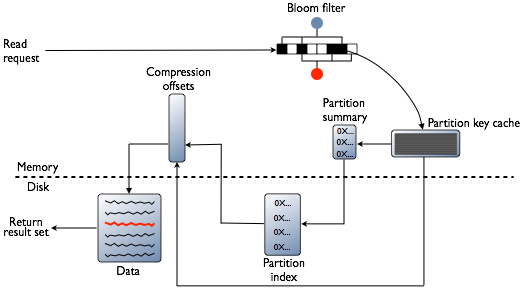
\includegraphics[width=0.75\textwidth]{resources/local_read.png}
  \end{center}

  Reading
\end{frame}

\subsection{How data is stored on disk}  % Erik

\begin{frame}{Sorted String Table (SSTable)}
  \begin{center}
    \Huge DEMO
  \end{center}
\end{frame}

\section{How the cluster works}  % Daniel

\begin{frame}{Token Ring}
  % http://abiasforaction.net/wp-content/uploads/2015/01/Cassandra-Ring.jpg
  \begin{columns}
    \begin{column}{0.6\textwidth}
    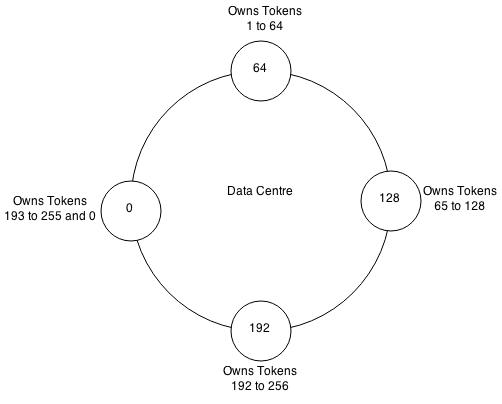
\includegraphics[width=\columnwidth]{resources/token_ring.jpg}
    \end{column}
    \begin{column}{0.4\textwidth}
      \begin{itemize}
        \item Num. Tokens $\propto$ Node Performance
        \item Hash(PartitionKey) \\ $\rightarrow$ Token
      \end{itemize}
    \end{column}
  \end{columns}
\end{frame}

\begin{frame}{Node joins or leaves ring - Rebalancing}
  \begin{itemize}
    \item Node joins ring $\rightarrow$ Joins at random location
    \item Node leaves ring $\rightarrow$ Leaves space on ring
  \end{itemize}
  % https://www.datastax.com/wp-content/uploads/2012/02/numofmoves.png
  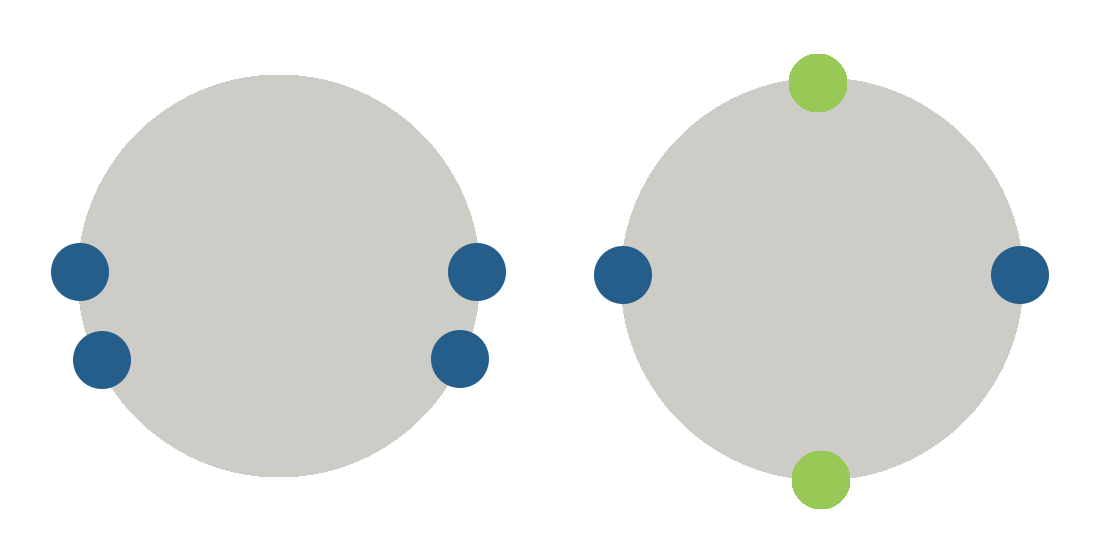
\includegraphics[width=\textwidth]{resources/rebalancing.png}
\end{frame}

\begin{frame}{Ring with replicas and virtual nodes}
  \begin{columns}
    \begin{column}{0.7\textwidth}
      % https://engineeringblog.yelp.com/images/posts/monitoring-cassandra-at-scale/cassandra_ring.png
      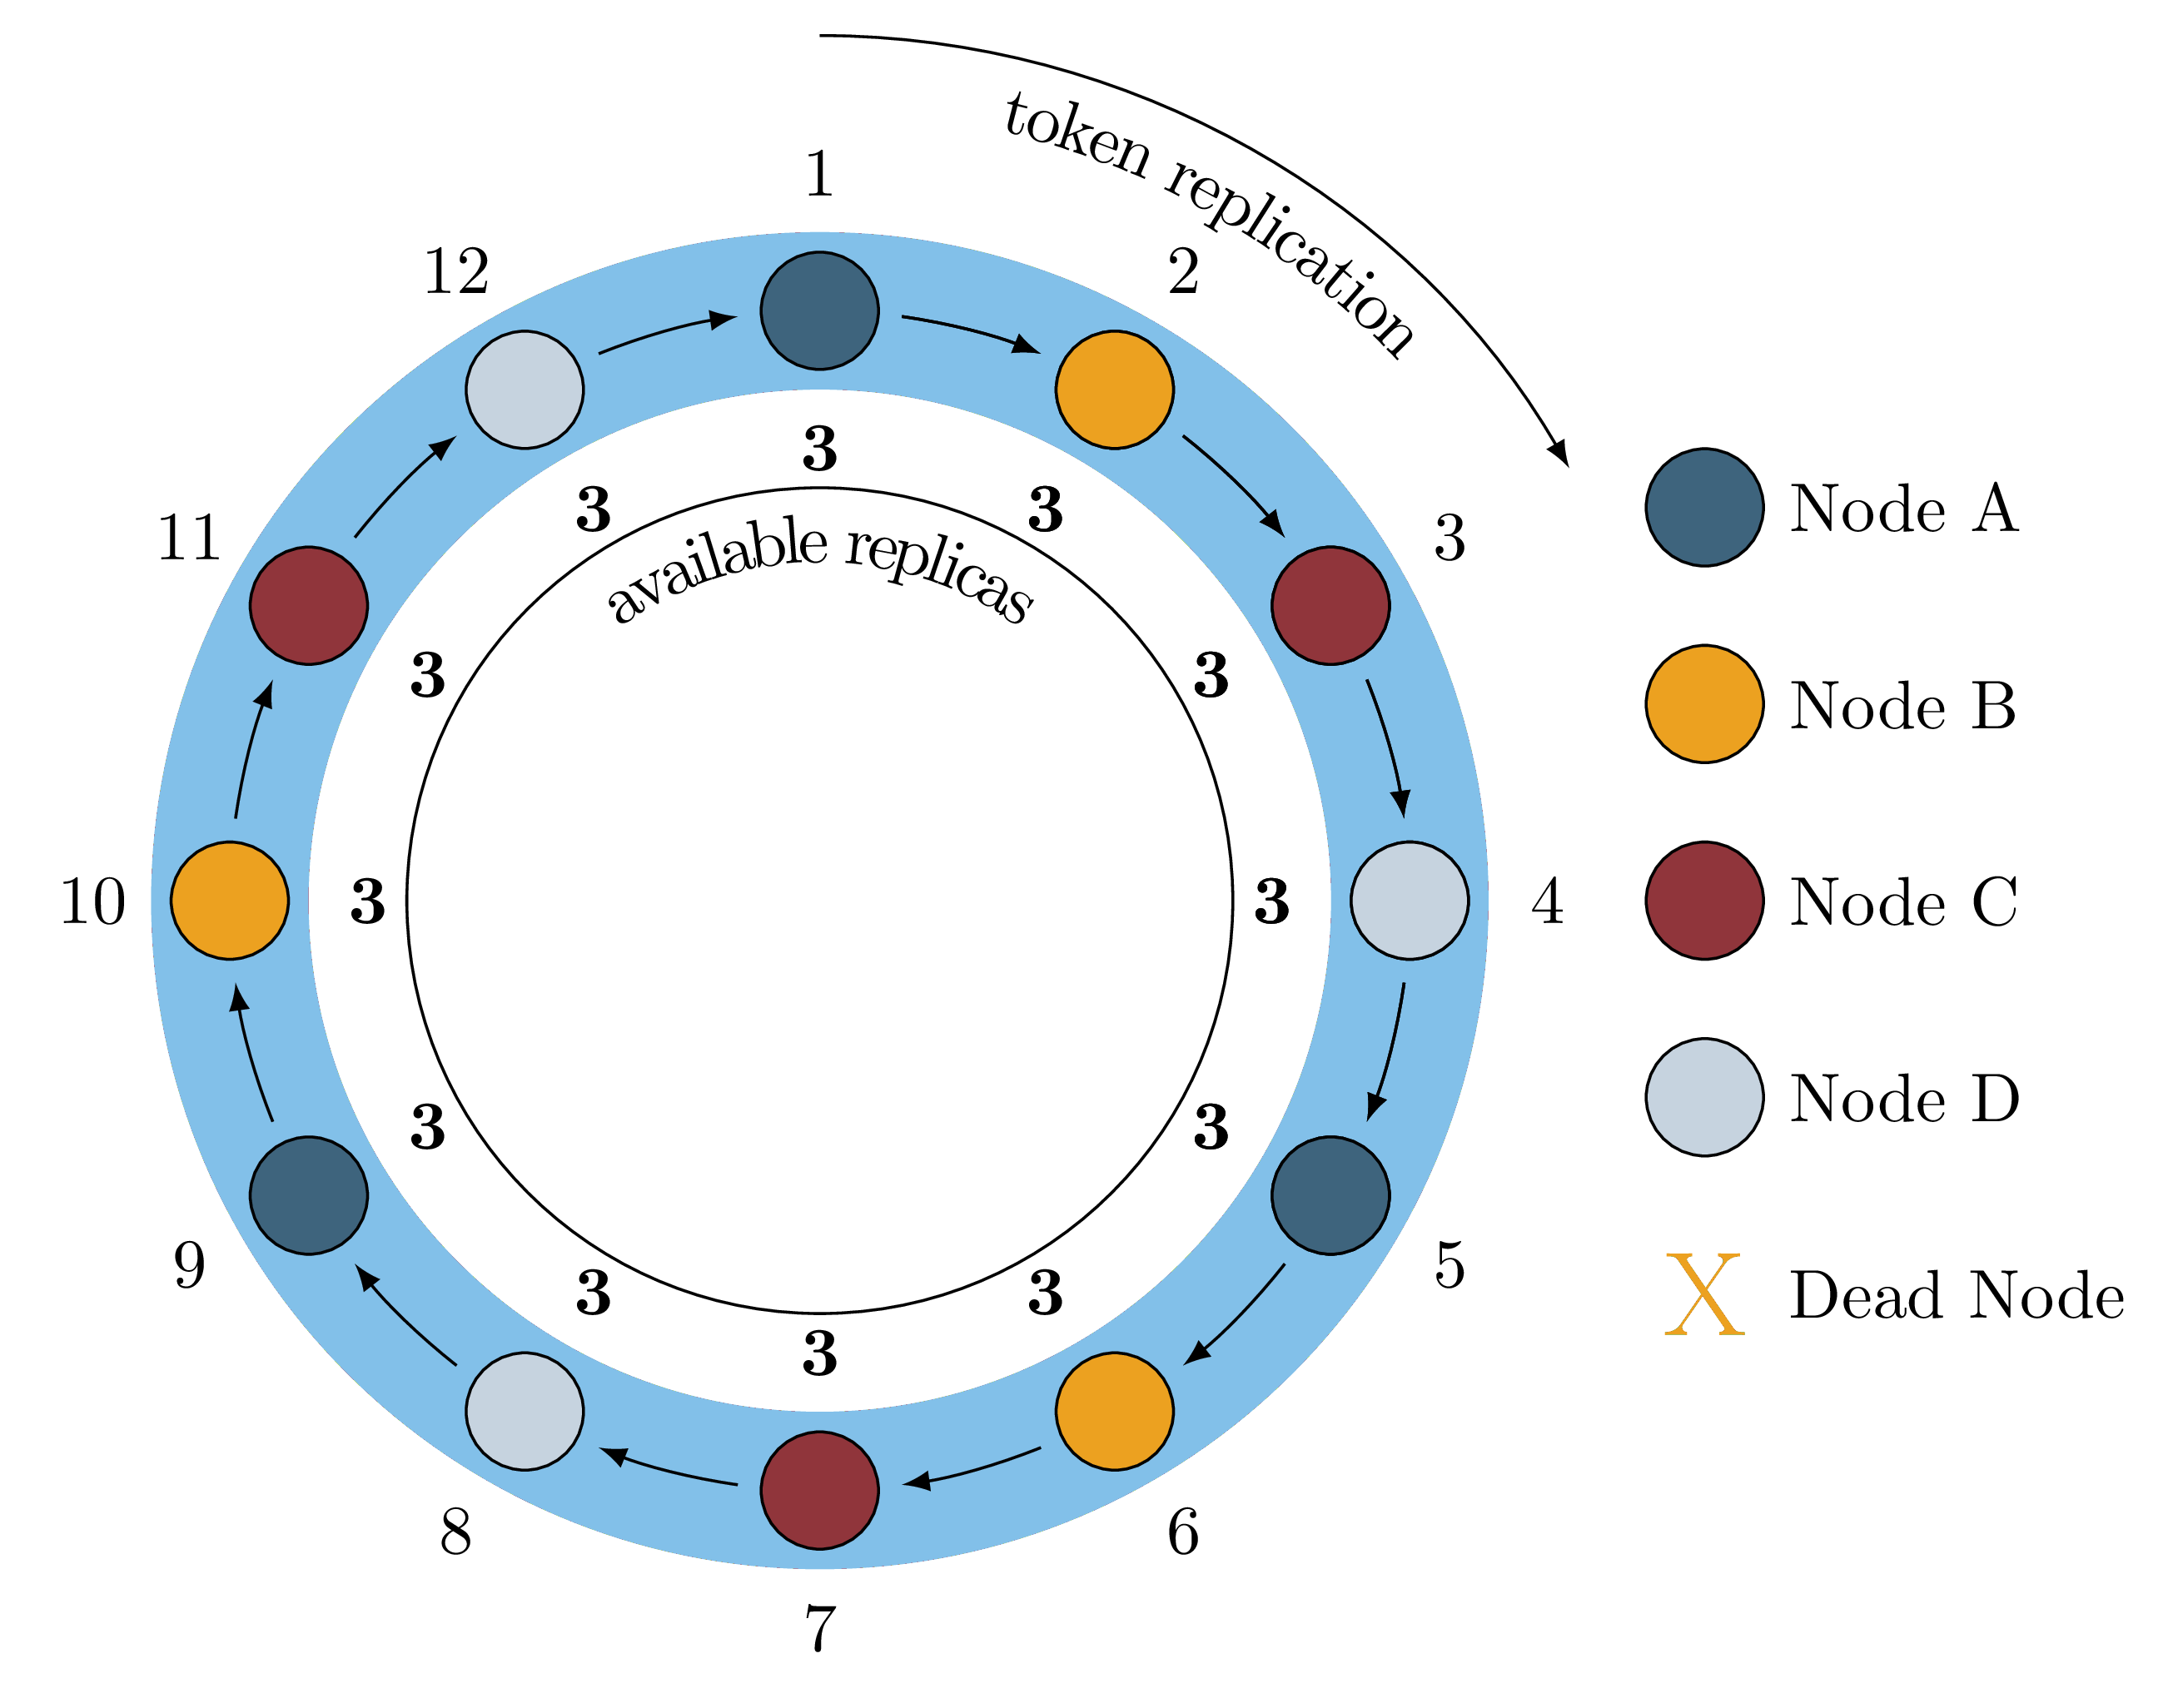
\includegraphics[width=1.0\textwidth]{resources/replica_ring.png}
    \end{column}
    \onslide<2->
    \begin{column}{0.3\textwidth}
      No
      \begin{itemize}
        \item Rebalancing
        \item Manual token calculation
      \end{itemize}
      Less
      \begin{itemize}
        \item Data hotspots
      \end{itemize}
    \end{column}
  \end{columns}
\end{frame}

\section{Distributed writes and reads (CAP)}  % Daniel

\begin{frame}{CAP Theorem}
  \begin{itemize}
    \item AP by default
    \item Can be tuned on a continuum towards CP
    \item AC not possible  % https://codahale.com/you-cant-sacrifice-partition-tolerance/
  \end{itemize}
\end{frame}

\begin{frame}{How data is replicated}
  % Draw manually if someone's bored
  % https://docs.datastax.com/en/cassandra/3.0/cassandra/images/arc_write-singleDCConOne.png
  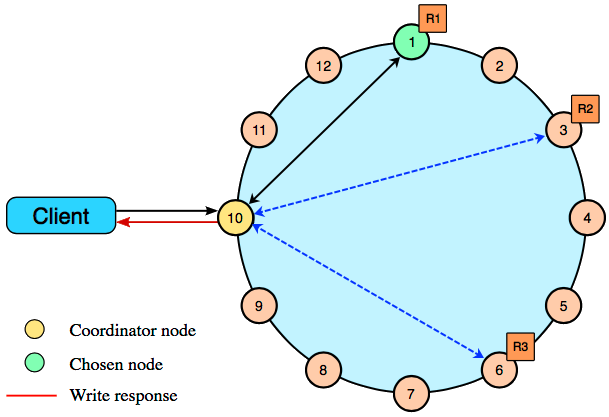
\includegraphics[width=1.0\textwidth]{resources/distributed_write.png}
\end{frame}

\begin{frame}{How data is replicated}
  % Can fail!
  \begin{enumerate}
    \item<1-> Client asks any node (becomes coordinator)
    \item<2-> Coordinator asks responsible nodes (replicas)
    \item<3-> When more than \lstinline{CL.write} nodes have confirmed write client is given answer
    \item<4-> Temporarily offline nodes are later reminded with a \textit{hinted-handoff}
  \end{enumerate}
\end{frame}

\begin{frame}{How data is replicated - Hinted Handoff}
  % https://docs.datastax.com/en/cassandra/3.0/cassandra/images/dml_hinted_handoff.png
  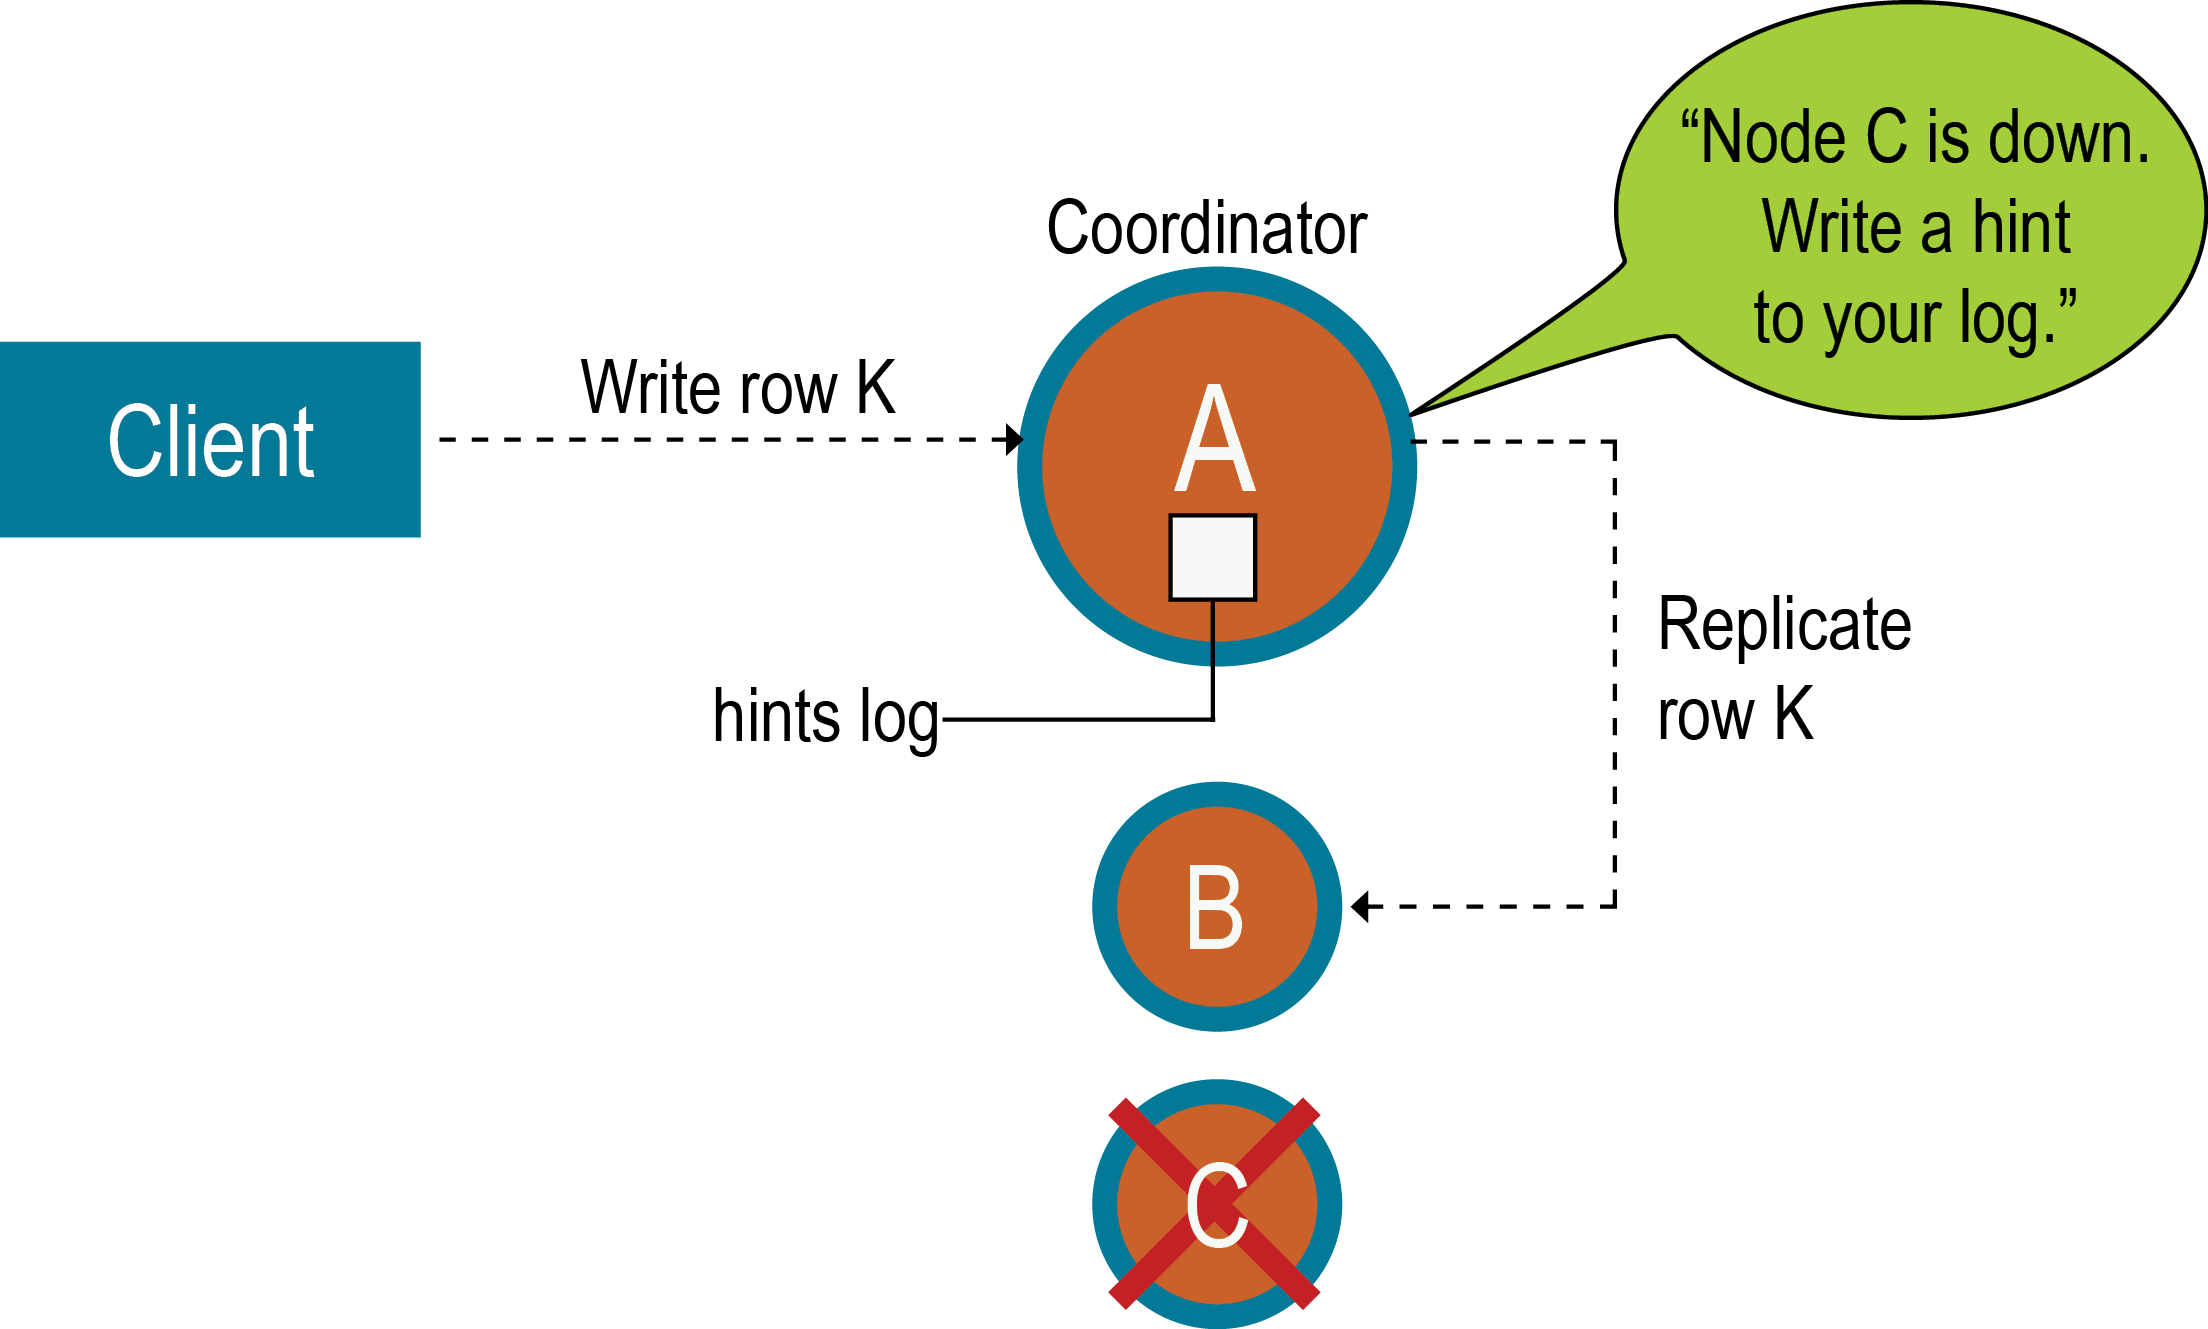
\includegraphics[width=1.0\textwidth]{resources/hinted_handoff.png}
\end{frame}

\begin{frame}{How data is read with consensus}
  \begin{enumerate}
    \item<1-> Client asks any node (becomes coordinator)
    \item<2-> Coordinator asks responsible nodes (replicas)
    \item<3-> When more than \lstinline{CL.read} nodes have answered client is given answer
    \item<4-> Nodes that sent outdated data are sent a \lstinline{read_repair}
  \end{enumerate}
\end{frame}

\begin{frame}{CAP Theorem - Tunable Variables}
  \begin{itemize}
    \item<+-> Consistency: (\lstinline{ANY} $\rightarrow$ \textbf{\lstinline{ONE}} $\rightarrow$ \lstinline{QUORUM} $\rightarrow$ \lstinline{ALL})
      \begin{itemize}
        \item \lstinline{CL.Read}
        \item \lstinline{CL.Write}
      \end{itemize}
    \item<+-> Availability:
      \begin{itemize}
        \item \lstinline{ReplicationFactor} (1 $\rightarrow$ \textbf{3} $\rightarrow$ nodes)
        \item More nodes
      \end{itemize}
  \end{itemize}
\end{frame}

\section{Setup}  % Daniel

\begin{frame}{Setup - overview}
  \begin{enumerate}
    \item<1-> Get enough nodes ($\geq3$ with $8+$ cores and 32GB RAM, lots of disk)
    % http://cassandra.apache.org/doc/latest/operating/hardware.html
    \item<2-> Set up network (each node with own IP reachable from the others)
    \item<3-> Adapt configuration files
    \item<4-> Open firewall for necessary ports
    \begin{itemize}
      \item 7000: node $\leftrightarrow$ node (\lstinline{storage_port})
      \item 9042: client $\leftrightarrow$ node (\lstinline{native_transport_port})
    \end{itemize}
    \item<5-> Start seed nodes and then other nodes
    \item<6-> Use \lstinline{nodetool} or \lstinline{cqlsh} to interact with the cluster
  \end{enumerate}
  \note<1>[item]{Number for recommended nodes from Apache}
  \note<1>[item]{ECC RAM and SSD are recommended}
  \note<1>[item]{DataStax recommends keeping data per node near or below 1 TB}
  % https://docs.datastax.com/en/dse-planning/doc/planning/planningHardware.html
  \note<2>[item]{Cloud is perfectly suited for this}
  \note<2>[item]{Two nodes cannot share a broadcast address (e.g. NAT)}
\end{frame}

\begin{frame}[fragile]{How to set up - Initial node}
  /etc/cassandra/cassandra.yaml
  \begin{semiverbatim}
# Opens socket on this address
listen_address: "192.168.0.2"
# Tells other nodes its reachable on this address
broadcast_address: "3.14.1.59"

seed_provider:
  - class_name: org.apache.cassandra.locator.SimpleSeedProvider
    parameters:
      - seeds "3.14.1.59"

# Enable client communication
start_native_transport: true
  \end{semiverbatim}
  \note[item]{Own broadcast address is in seeds $\rightarrow$ Creates own cluster}
  \note[item]{For single node cluster use \lstinline{localhost} everywhere}
\end{frame}

\begin{frame}[fragile]{How to set up - Further nodes}
  /etc/cassandra/cassandra.yaml
  \begin{semiverbatim}
# Opens socket on this address
listen_address: "\textbf{192.168.1.2}"
# Tells other nodes its reachable on this address
broadcast_address: "\textbf{6.28.3.18}"

seed_provider:
  - class_name: org.apache.cassandra.locator.SimpleSeedProvider
    parameters:
      - seeds "3.14.1.59"

# Enable client communication
start_native_transport: true
  \end{semiverbatim}
  \note[item]{Seeds is a comma separated "list" of IPs}
  \note[item]{Three per datacenter recommended}
\end{frame}

\begin{frame}{More configuration}
  \begin{itemize}
    \item Tune JVM parameters like heap size in \lstinline{cassandra-env.sh}
    \item Increase the number of tokens (virtual nodes) with \lstinline{num_tokens}
    \item Other performance, architecture or security tuning
  \end{itemize}
\end{frame}

\begin{frame}{Security}
  \begin{itemize}
    \item<1-> Use a firewall to not expose it to the public internet
    \item<2-> Internode communication with TLS
    \item<2-> Client $\leftrightarrow$ Node communication with TLS
    \item<3-> JMX management only on localhost and with auth
    \item<4-> Authentication with password
    \item<5-> Disable default role
    \item<5-> Use roles
  \end{itemize}
  \note<1>[item]{Basic linux due diligence}
  \note<2>[item]{TLS is always good $\rightarrow$ Encryption, Authenticity}
  \note<5>[item]{There are no users, only roles (good RBAC model)}
\end{frame}

%\subsection{Things to keep in mind}
% How to set up as an admin / Must knows

\section{Summary and Conclusion}

\begin{frame}{Summary and Conclusion}
  \begin{itemize}
    \item<+-> Useful for \textit{logging} large amounts of data (Big Data)
    \item<+-> Highly available
    \item<+-> Not a replacement for RDBMS
    \item<+-> Sophisticated architecture
    \item<+-> Battle tested
    \item<+-> Fantastic for the use-cases its designed for
  \end{itemize}
\end{frame}

\begin{frame}{The end}
  \begin{columns}
    \begin{column}{0.5\textwidth}
      % https://upload.wikimedia.org/wikipedia/commons/thumb/5/5e/Cassandra_logo.svg/1920px-Cassandra_logo.svg.png
      
\includegraphics[width=\columnwidth]{resources/cassandra_logo.png}
    \end{column}
    \begin{column}{0.5\textwidth}
      Thank you for listening! \\
      Any questions?
    \end{column}
  \end{columns}
\end{frame}

\appendix

\begin{frame}{Comparison - Other Wide Column Datastores}
  \begin{center}
    \begin{tabular}{l|l}
      Name & Description \\
      \hline
      Amazon DynamoDB & Amazon makes the decisions for you \\
      % Original developers of DynamoDB created Cassandra
      % Easy but less tunable
      % MultiCloud, Partitions, Nodes, Consistency level, ...
      % Cassandra based off of DynamoDB
      Google BigTable & Based on GFS (CP), Managed by Google \\
      % Can be used with Cassandra like architecture (default)
      ScyllaDB & Cassandra rewrite with better performance \\
      % C++ and better handling of multiple requests
      % Not yet all features and not "battle tested"
      Apache HBase & Similar data model, master/slave $\rightarrow$ CP\\
    \end{tabular}
  \end{center}
\end{frame}

\end{document}
